%%%%%%%%%%%%%%%%%%%%%%%%%%%%%%%%%%%%%%%%%
%
% (c) 2021 by Jennifer Laaser
%
% This work is licensed under the Creative Commons Attribution-NonCommercial-ShareAlike 4.0 International License. To view a copy of this license, visit http://creativecommons.org/licenses/by-nc-sa/4.0/ or send a letter to Creative Commons, PO Box 1866, Mountain View, CA 94042, USA.
%
% The current source for these materials is accessible on Github: https://github.com/jlaaser/pogil-polymers
%
%%%%%%%%%%%%%%%%%%%%%%%%%%%%%%%%%%%%%%%%%

\renewcommand{\figpath}{content/polymphys/chain-confs/chain-models/figs}
\renewcommand{\labelbase}{chain-models}

\begin{activity}{Models for Polymer Chains}

\begin{instructornotes}

	This activity introduces students to the concept of conformations of polymer chains.
	
	After completing this activity, students will be able to:
			\begin{enumerate}
				\item \dots
			\end{enumerate}
	
			
	\subsection*{Activity summary:}
	\begin{itemize}
		\item \textbf{Activity type:} Learning Cycle
		\item \textbf{Content goals:} Basics of Chain Conformations
		\item \textbf{Process goals:} %https://pogil.org/uploads/attachments/cj54b5yts006cklx4hh758htf-process-skills-official-pogil-list-2015-original.pdf
			\begin{itemize}
				\item %Connecting key relationships to derive a result
				\item %Interpreting mathematical equations in terms of physical behavior
				\item %Oral and written communication of reasoning
			\end{itemize}
		\item \textbf{Duration:} approx. ??? minutes, including time for class discussion
		\item \textbf{Instructor preparation required:} 
			\begin{itemize}
				\item None beyond knowledge of relevant content
			\end{itemize}
		\item \textbf{Related textbook chapters:}
			\begin{itemize}
				\item \emph{Polymer Chemistry} (Hiemenz \& Lodge): Section ???
			\end{itemize}
	\end{itemize}

\end{instructornotes}

	%\textbf{Focus question:} Put a central question for the students to consider through this exercise here.

\begin{model}[Random Walks]
\label{\labelbase:mdl:randomwalks}

	The simplest model for a polymer chain is a \emph{freely-jointed chain} consisting of $n$ links of length $l$ that can each point in any direction, regardless of the direction of the previous link.
	
	To understand the properties of a freely-jointed chain, we will first consider a simple one-dimensional model in which each link can point either to the right or the left with equal probability.

\end{model}


\begin{ctqs}

	\question Suppose the beginning of the chain is at $x=0$, and each link has length $l=1$.
	
		\begin{enumerate}
			\item What is the probability that, after the first link, you are at position $x=1$?
			
				\emph{(Hint: remember that each link has an equal probability of pointing to the right or to the left!)}
				
				\begin{solution}[0.5in]
				\end{solution}
				
			\item Similarly, what is the probability that, after the first link, you are at position $x=-1$?
				
				\begin{solution}[0.5in]
				\end{solution}
			
		\end{enumerate}
		
	\question Building off your answers to the previous question, what are the probabilities that after the \emph{second} link you will be at...
	
		\begin{enumerate}
			
			\item ... position $x=2$?
			
				\emph{(Hint: remember that to get a total probability, we \emph{multiply} the probabilities of each step leading to the final outcome.)}
				
				\begin{solution}[1in]
				\end{solution}
				
			\item ... position $x=-2$?
				
				\begin{solution}[1in]
				\end{solution}
			
			\clearpage
			\item ... position $x=0$?
				\emph{(Hint: how many ways could you get to this final position?)}
				
				\begin{solution}[1in]
				\end{solution}
			
		\end{enumerate}
		
	\question Plot the probabilities you calculated in the previous question on the axes below:
	
		\vspace{24pt}
		\centerline{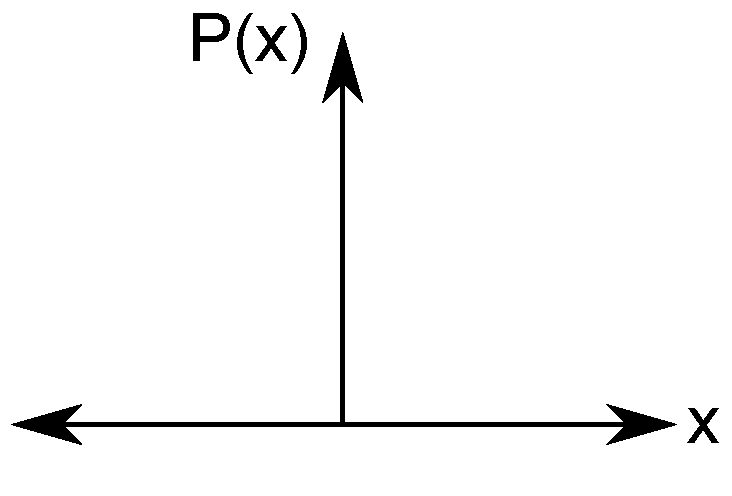
\includegraphics[width=0.5\textwidth]{\figpath/Model1_probability_axes}}
	
	\question Predict what the probability distribution might look like after 100 links:
	
		\vspace{24pt}
		\centerline{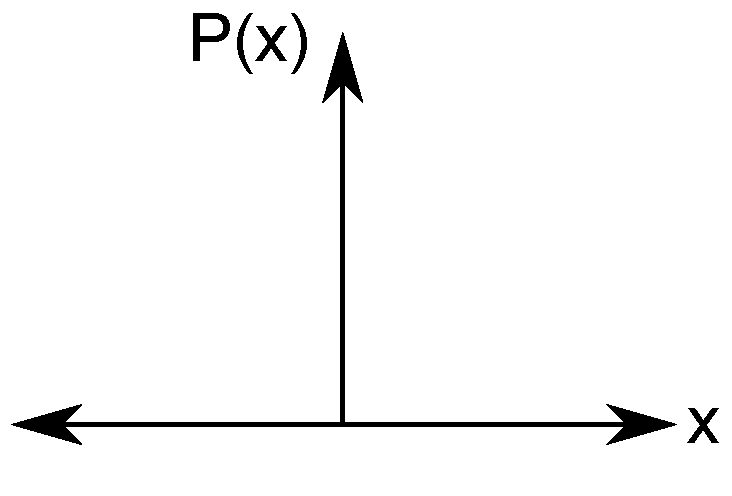
\includegraphics[width=0.5\textwidth]{\figpath/Model1_probability_axes}}
	
\end{ctqs}

\begin{infobox}
	
	The process you have investigated in the previous questions is called a \emph{random walk}.
	
	It is possible to show that after $n$ steps, the probability of being at position $x$ is approximately
	\begin{equation*}
		P(n,x) = \frac{1}{\sqrt{2\pi n}}e^{-x^2/2n}
	\end{equation*}
	
\end{infobox}

\begin{ctqs}

	\question As you know, in polymer science, we usually have to calculate \emph{average} properties over all of the possible conformations of the polymer chains.
	
		The average value of any function of $x$, $\langle f(x)\rangle$, can be calculated using
		\begin{equation*}
			\langle f(x) \rangle = \int_{-\infty}^\infty f(x) P(n,x)\,dx
		\end{equation*}
		
		\begin{enumerate}
			\item Evaluate the average final position, $\langle x \rangle$, for the 1D random walk described above.
			
				\emph{Hint: you will probably find one of the following integrals useful:}
				\begin{align*}
					\int_{-\infty}^\infty e^{-a x^2} = \sqrt{\frac{\pi}{a}} && \int_{-\infty}^\infty x e^{-a x^2} = 0 && \int_{-\infty}^\infty x^2 e^{-a x^2} = \frac{1}{2}\sqrt{\frac{\pi}{a^3}}
				\end{align*}
				
				\begin{solution}[1.5in]
				\end{solution}
				
			\item Why is $\langle x \rangle$ not a particularly useful way to describe the properties of a polymer chain?  Explain your group's reasoning in 1-2 complete sentences.
				
				\begin{solution}[1.5in]
				\end{solution}
			
		\end{enumerate}
		
	\question Suppose you instead wanted to calculate the mean square end-to-end distance of your chain, $\langle x^2\rangle$.
	
		\begin{enumerate}
			\item Write down an appropriate integral for this quantity and evaluate it as above.
				
				\begin{solution}[1.5in]
				\end{solution}
			
			\item Is $\langle x^2 \rangle$ a more useful measure of the size of a polymer chain?  Explain your group's reasoning in 1-2 complete sentences.
				
				\begin{solution}[1.5in]
				\end{solution}
		\end{enumerate}
		

\end{ctqs}

\begin{model}[Models for Polymer Chains]
\label{\labelbase:mdl:chainmodels}

	As noted in Model \ref{\labelbase:mdl:randomwalks}, the simplest model for a polymer chain is one in which each link can point in any direction, regardless of the direction of the previous link.
	
	This model is called a \emph{freely-jointed} chain, and it is possible to show that the mean square end-to-end distance for a freely-jointed chain is given by
	\begin{equation*}
		\langle h^2\rangle =nl^2
	\end{equation*}
	
	Real polymers, however, are not freely-jointed, because chemical bonds cannot, realistically, bend to any arbitrary angle.
	
	Two more chemically-reasonable models for polymer chains are:
	
	\begin{enumerate}
		\item The \emph{freely-rotating} chain.  In this model, the bond angle $\theta$ is fixed, but the rotation angle $\phi$ can take any value:
		
			\begin{minipage}[t]{0.45\textwidth}
				\vspace{1in}~
			\end{minipage}%
			\begin{minipage}[t]{0.45\textwidth}
				\begin{equation*}
					\langle h^2\rangle = n l^2 \left[\frac{1+\cos\theta}{1-\cos\theta}\right]
				\end{equation*}
			\end{minipage}
		
		\item The \emph{hindered-rotation} chain.  In this model, the bond angle $\theta$ is fixed, and some rotation angles $\phi$ are more favorable than others (e.g. because of sterics within the molecule):
		
			\begin{minipage}[t]{0.45\textwidth}
				\vspace{1in}~
			\end{minipage}%
			\begin{minipage}[t]{0.45\textwidth}
				\begin{equation*}
					\langle h^2\rangle = n l^2 \left[\frac{1+\cos\theta}{1-\cos\theta}\right] \left[\frac{1+\langle \cos\phi\rangle}{1-\langle\cos\phi\rangle}\right]
				\end{equation*}
			\end{minipage}
			
	\end{enumerate}
	
\end{model}

\begin{ctqs}
	\question For a chain with $n$ links of length $l$, which of these models do you expect to produce the most extended chain conformation?  Explain your group's reasoning in 2-3 complete sentences. \label{\labelbase:ctq:stiffness}
	
		\begin{solution}[1.5in]
		\end{solution}
	
	\question If you look closely, you should notice that for each of these models, $\langle h^2\rangle$ can be written in the form \label{\labelbase:ctq:C}
		\begin{equation*}
			\langle h^2 \rangle = C_\infty n l^2
		\end{equation*}
		
		Write an expression for the characteristic ratio, $C_\infty$, for...
		
		\begin{enumerate}
			\item ... the freely-jointed chain:
	
		\begin{solution}[0.75in]
		\end{solution}
			
			\item ... the freely-rotating chain:
	
		\begin{solution}[0.75in]
		\end{solution}
			
			\item ... the hindered-rotation chain:
	
		\begin{solution}[0.75in]
		\end{solution}
		\end{enumerate}
		
\end{ctqs}

\begin{infobox}

A quantitative measure of a polymer's stiffness is its \emph{persistence length}, which tells you how far you have to go along the polymer backbone before the chain, on average, turns by 90$^\circ$.
	
		The persistence length is given by
		\begin{equation*}
			l_p = C_\infty \frac{l}{2}
		\end{equation*}
		
\end{infobox}

\begin{ctqs}

	\question Is this information consistent with your answers to questions \ref{\labelbase:ctq:stiffness} and \ref{\labelbase:ctq:C}?
	
		\begin{solution}[0.75in]
		\end{solution}
	
	\question The equations given in Model \ref{\labelbase:mdl:chainmodels} express the chain dimensions in terms of the number of bonds $n$ and the bond length $l$.  However, it is often also useful to describe a polymer in terms of the ``closest equivalent'' freely-jointed chain.
	
		\begin{enumerate}
			\item  If the ``closest equivalent'' freely-jointed chain has $N$ links of length $b$, how long would the chain be if it were fully extended? \label{\labelbase:ctq:Nb}
	
		\begin{solution}[0.75in]
		\end{solution}
			
			\item What would the mean-square end-to-end distance of the chain be? \label{\labelbase:ctq:Nb2}
	
		\begin{solution}[0.75in]
		\end{solution}
			
			\item Combine your answers from parts \ref{\labelbase:ctq:Nb} and \ref{\labelbase:ctq:Nb2} to find expressions for $N$ and $b$ in terms of the characteristic ratio $C_\infty$, the number of bonds $n$, and the bond length $l$.
	
		\begin{solution}[1.25in]
		\end{solution}
		\end{enumerate}
		
	\question The link length $b$ is called the \emph{statistical segment length}.  Does the statistical segment length have a simple physical interpretation?  Briefly explain your group's reasoning in 2-3 complete sentences.
	
		\begin{solution}[1.5in]
		\end{solution}
	
	\question Finally, in many experiments, it is easier to measure the \emph{radius of gyration} for a polymer chain (the mean square distance between the monomers and the polymer's center of mass), $R_g$.  For the ideal chains described in Model \ref{\labelbase:mdl:chainmodels}, it can be shown that
		\begin{equation*}
			\langle R_g^2\rangle = \frac{\langle h^2\rangle}{6}
		\end{equation*}
		
		\begin{enumerate}
			\item Find an expression for $\langle R_g^2 \rangle$ in terms of $N$ and $b$.
	
		\begin{solution}[1in]
		\end{solution}
			
			\item If you were to double the length of the chain, by what factor would you expect the radius of gyration to increase?
	
		\begin{solution}[1in]
		\end{solution}
			
			\item Explain, in 1-2 complete sentences, why we might say that the radius of gyration ``scales as'' the square root of the chain length.
	
		\begin{solution}[1.5in]
		\end{solution}
		\end{enumerate}
	
\end{ctqs}

%\begin{model}[Radius of Gyration]
%	\label{\labelbase:mdl:Rg}
%	...
%\end{model}
	
	
\begin{exercises}
	\exercise A useful rule of thumb for calculating radius of gyration is that the radius of gyration for polymers with a molecular weight of $10^5$ g/mol is typically about 10~nm.
	
		\begin{enumerate}
			\item Predict the radius of gyration of a polymer with a molecular weight of $2\times10^5$~g/mol.
			
			\item Predict the molecular weight of a polymer with a radius of gyration of 100~nm.
		\end{enumerate}
\end{exercises}
	
\end{activity}